\chapter{DevOps}
\authors{Hendra Lijaya, Oktavianus Hendry Wijaya}

\section{Pengertian}
DevOps merupakan metode pengembangan software dengan mengkolaborasikan \textit{software developer} dengan \textit{IT operation}. 
\section{Fungsi}
Tujuan akhir atau \textit{goal} dari DevOps adalah untuk menciptakan lingkungan kolaborasi yang berkelanjutan untuk membawa software menjadi lebih berkualitas, lebih cepat, dan dapat diandalkan.
\begin{figure}[h]
	\centering
	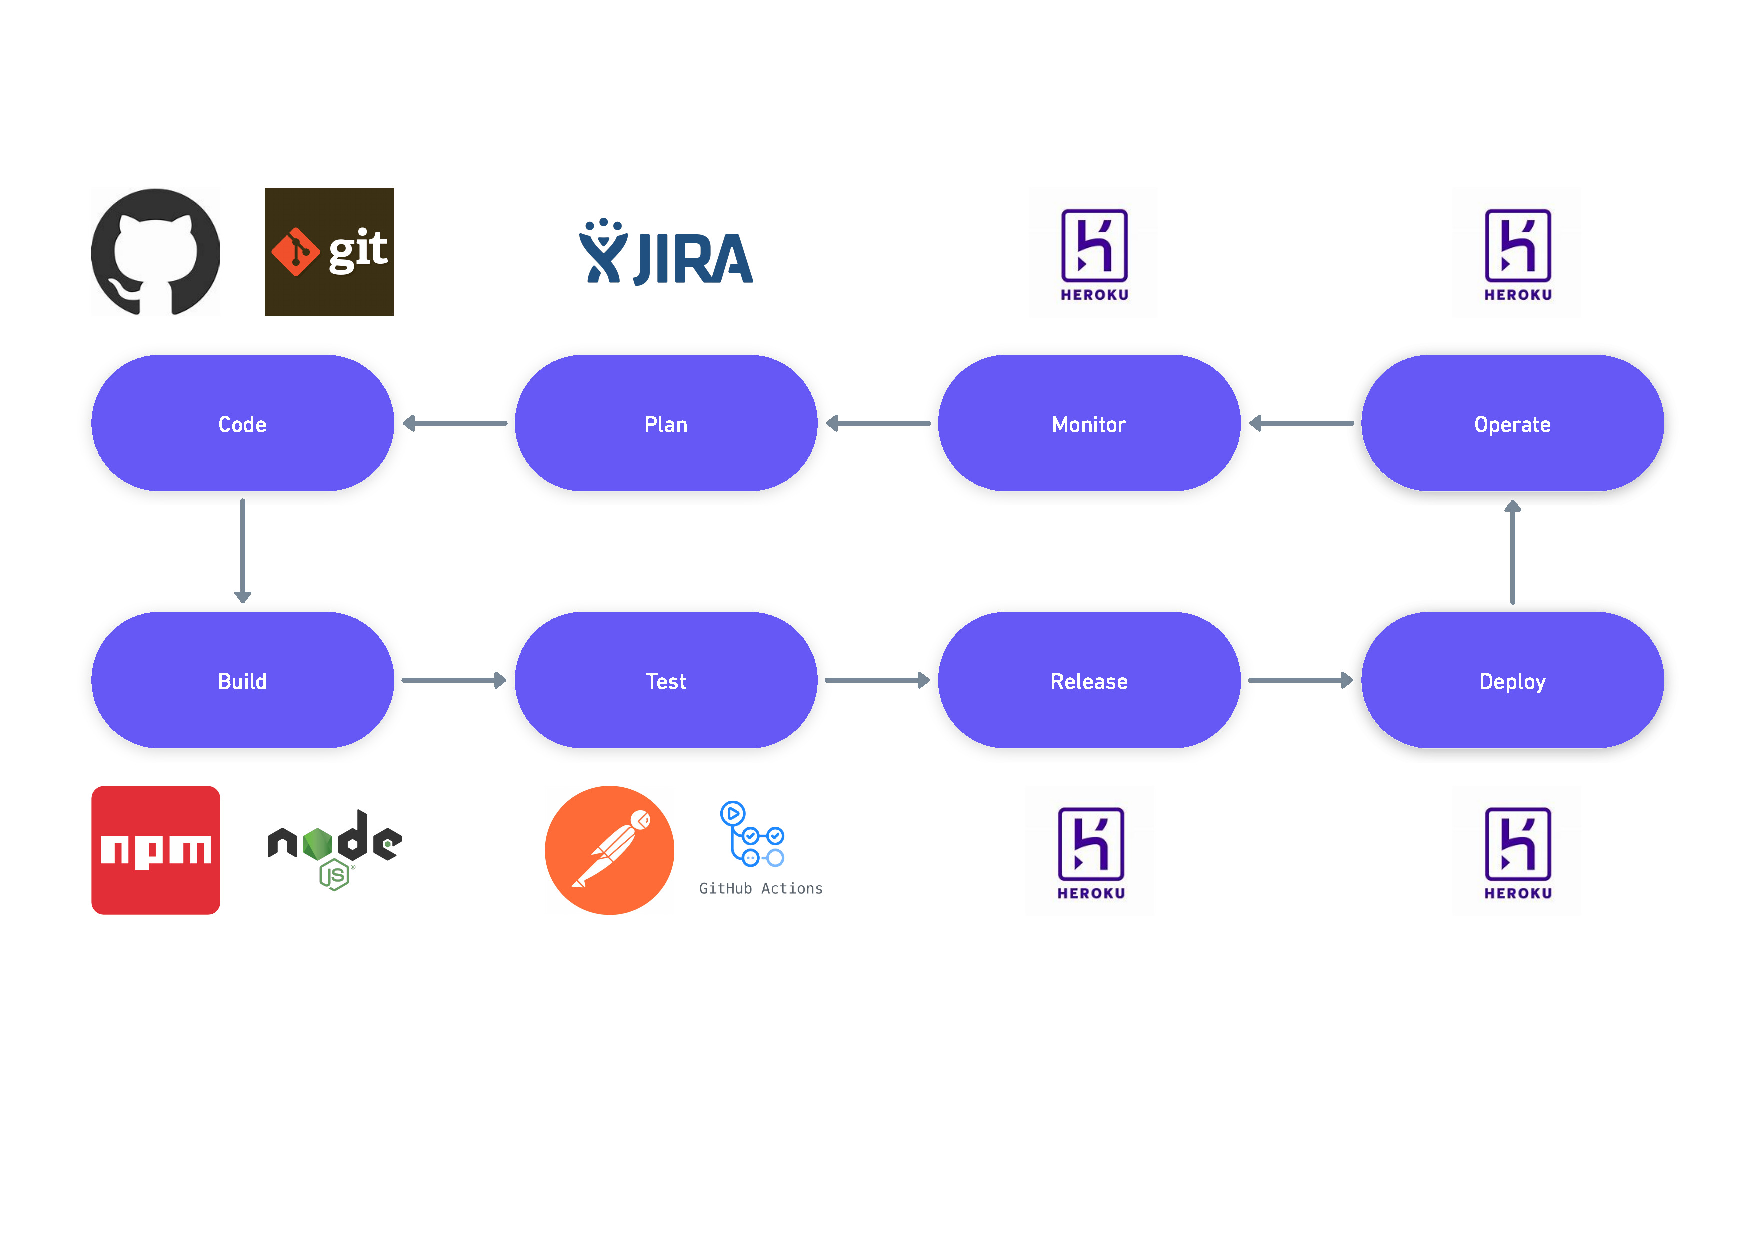
\includegraphics[width=\textwidth]{../images/Arsitektur DevOps}
	\caption{Arsitektur DevOps.}
	\label{fig:Arsitektur DevOps}
\end{figure}
\section{Arsitektur}
	\begin{itemize}
	\item \textit{Plan}
	\\Tahap paling awal dalam SDLC (\textit{Software Development Life Cycle}). Mulai dari tahap pengumpulan data, membuat \textit{roadmap}, menetapkan tujuan, \textit{timelines} serta mengidentifikasi \textit{resources} yang diperlukan untuk menyelesaikan sebuah proyek.
	\item \textit{Code}
	\\Pada tahap ini, developer mulai menulis kode untuk mengembangkan \textit{software} berdasarkan requirement yang telah dikumpulkan pada tahap \textit{Plan}.
	\item \textit{Build}
	\\Pada tahap ini, kode di \textit{compile}, dan di \textit{package} kedalam format yang bisa di \textit{deliver}. Tujuan tahap ini membuat kode yang telah di \textit{compile} agar dapat melakukan tahap \textit{Testing} dan \textit{Release}.
	\item \textit{Test}
	\\Pada tahap ini, perangkat lunak diuji untuk memastikan bahwa perangkat lunak sudah memenuhi requirement dan fungsinya sudah berjalan tanpa ada \textit{bug}.
	\item \textit{Release}
	\\Pada tahap ini, perangkat lunak sebelum di \textit{deploy} ke \textit{staging} atau \textit{production} \textit{environment} dapat dilakukan data migrasi, konfigurasi dan lainnya. Tujuannya adalah untuk memastikan bahwa perangkat lunak tersedia dan dapat digunakan oleh audiens yang dituju.
	\item \textit{Deploy}
	\\Pada tahap ini, perangkat lunak di \textit{deploy} ke \textit{production} ataupun \textit{staging} bisa menggunakan tools atau \textit{automation} \textit{script}. Proses ini mencakup juga instalasi library, dan konfigurasi server dan lainnya.
	\item \textit{Operate}
	\\Pada tahap ini, perangkat lunak sudah beroperasi di \textit{production environment} dan dapat dikelola dan dipantau untuk memastikan kinerjanya seperti yang diharapkan.
	\item \textit{Monitor}
	\\Pada tahap ini, pengumpulan dan analisis data dari log sistem. Informasi ini dapat digunakan untuk mengidentifikasi area untuk perbaikan, mengoptimalkan kinerja, dan menginformasikan upaya pengembangan perangkat lunak kedepannya.
\end{itemize}



\section{Kelebihan Kekurangan}
Berikut adalah kelebihan dan kekurangan arsitektur DevOps:

\subsection{Kelebihan}
Keuntungan dari menerapkan arsitektur DevOps adalah:
\begin{itemize}
	\item DevOps menjadi pilihan yang bagus untuk \textit{development} dan \textit{deployment} aplikasi yang cepat
	\item Merespon lebih cepat ke perubahan market untuk meningkatkan \textit{business growth} (pertumbuhan bisnis)
	\item Data dapat disentralisasikan sehingga meningkatkan konsistensi data dan mengurangi duplikasi data.
	\item DevOps meningkatkan profit bisnis dengan mengurangi waktu \textit{delivery software} dan biaya.
	\item DevOps menghilangkan proses deskriptif sehingga memberikan kejelasan mengenai \textit{development} dan \textit{delivery product}.
	\item Meningkatkan \textit{experience} dan kepuasan \textit{customer}.
	\item DevOps menyederhanakan kolaborasi dan menggunakan semua \textit{tools} di cloud untuk diakses pengguna.
	\item Meningkatkan keterlibatan dan produktivitas tim.
\end{itemize}
\subsection{Kekurangan}
Kekurangan dari penerapan arsitektur DevOps adalah:
\begin{itemize}
	\item DevOps \textit{professional} atau \textit{expert} masih belum umum ditemukan.
	\item \textit{Developing} dengan DevOps mahal.
	\item Penerapan DevOps baru ke dalam industri sulit untuk dikelola dalam waktu singkat.
	\item 	Kurangnya pengetahuan mengenai DevOps dapat menyebabkan masalah pada \textit{Continuous Integration} dari \textit{project automation}.
\end{itemize}
\section{Perbedaan DevOps dan nonDevOps}
Perbedaan besar dari \textit{development} dengan DevOps dan nonDevOps yaitu:
	\begin{enumerate}
		\item Kolaborasi
		\\Pada \textit{Software development} nonDevOps, developer dan tim operation bekerja secara terpisah. Sedangkan pada DevOps, kedua hal tersebut bekerja secara kolaboratif dalam 2 tim yang berbeda dengan berbagi pengentahuan dan skill sehingga memastikan proses software development dapat disederhanakan.
		
		\item \textit{Continuous Integration and Delivery (CI/CD)}
		\\DevOps menerapkan CI/CD yang dimana melibatkan sistem \textit{automation} pada proses \textit{software development} mulai dari \textit{building} dan \textit{testing} hingga ke \textit{deployment} dan \textit{maintenance}. Dengan menerapkan ini, perubahan dapat di tes dan diintegrasikan ke software secara cepat dan efisien mungkin.
		\item \textit{Automation}
		\\DevOps bergantung secara penuh pada automation untuk meningkatkan efisiensi dan mengurangi error. Tools seperti \textit{management configuration}, \textit{continuous integration}, dan \textit{continuous delivery} memungkinkan tim untuk mengautomatis proses yang awalnya manual dan memastikan konsistensi.
		\item \textit{Monitoring}
		\\Tim yang menerapkan DevOps menggunakan \textit{tools} untuk \textit{monitoring} dan analitik untuk mengumpulkan data mengenai performa pada software saat \textit{production}. Hal ini membantu tim dalam mengidentifikasi dan menyelesaikan isu dengan cepat sehingga mengurangi downtime dan meningkatkan \textit{user experience} secara keseluruhan.
		\item Agile Development
		\\DevOps berdasarkan pada prinsip \textit{agile development} yang dimana fleksibilitas, adaptabilitas, dan kolaborasi sangat ditekankan. Tim DevOps memprioritaskan dalam \textit{delivery} dalam perubahan kecil dan perubahan \textit{incremental} dengan cepat dibandingkan perilisan monolitik yang bersifat besar.
	\end{enumerate}
	Kesimpulannya adalah DevOps bersifat lebih kolaboratif, \textit{automated}, dan \textit{agile} pada proses\textit{ software development} yang menekankan \textit{continuous integration and delivery, automation, }dan \textit{monitoring}.

\section{Tools}
Tools yang digunakan dalam pembuatan DevOps:
\begin{enumerate}
	\item Git - GitHub Action
	\\GitHub Action adalah fitur dari \textit{platform} GitHub yang memungkinkan developer untuk mengautomasi \textit{workflows} dan \textit{build, test}, dan \textit{deploy} kode langsung  dari \textit{platform} GitHub.
	GitHub Action menyediakan \textit{library} dari \textit{pre-built actions }yang dapat digunakan untuk membangun \textit{workflows} dan juga kemampuan untuk membuat action kustom menggunakan JavaScripts atau Docker containers. \textit{Workflows} dapat dipicu/di\textit{trigger} oleh \textit{events} seperti push kode, request pull, atau pembuatan perilisan baru.
	\\Keuntungan menggunakan GitHub:
	\begin{itemize}
		\item Terintegrasi dengan GitHub
		\item Workflows yang dapat dikustomisasi
		\item Reusability
		\item Kolaborasi
		\item Skalabilitas
		\item Gratis
	\end{itemize}
	Kesimpulan, GitHub Action merupakan \textit{tools} yang sangat berguna untuk \textit{automating software development workflows}, menyediakan developer fleksibilitasm, kustomisasi, dan platform yang terintegrasi untuk \textit{building, testing,} dan \textit{deploy} kode
	
	\item Heroku
	\\Heroku merupakan \textit{platform cloud} yang memungkinkan developer untuk \textit{build, deploy}, dan mengelola aplikasi secara cepat dan mudah. Heroku mendukung beberapa Bahasa pemrograman seperti Java, Ruby, Node.js, Python, PHP, dan Go. Heroku menyediakan platform yang dikelola secara penuh sehingga developer tidak perlu mengkhawatirkan mengenai mengelola infrastruktur, sistem operasi, dan server.
	\\Heroku didasarkan pada arsitektur yang berbasis \textit{container} dan menggunakan Dyno untuk menjalankan aplikasi. Dyno merupakan \textit{container} linux yang ringan dan terisolasi yang berjalan diatas platform Heroku. Dyno di\textit{design} untuk menjalankan satu proses atau layanan yang membantu meningkatkan performa, skalabilitas, dan ketahanan.
	\\Fitur-fitur Heroku:
	\begin{itemize}
		\item \textit{Command Line Interface }(CLI)
		\item \textit{Web Based Dashboard}
		\item Beragam \textit{add-ons} dan \textit{extensions}
		\item\textit{ Support continuous integration and continuous delivery (CI/CD) workflows}.
	\end{itemize}
	Adapun kekurangan dari Heroku yaitu:
	\begin{itemize}
		\item Kustomisasi yang terbatas.
		\item Bergantung pada \textit{add-on third party}.
		\item Memerlukan biaya dan kartu kredit.
	\end{itemize}

	\item Postman
	\\Postman merupakan tools software yang sering digunakan oleh developer untuk \textit{test}, dokumentasi, dan berbagi API. API atau \textit{Application Programming Interfaces} memungkinkan software aplikasi yang berbeda untuk berkomunikasi melalui pertukaran data antara satu dengan yang lain.
	\\Dengan menggunakan Postman, developer dapat dengan mudah membuat dan mengeksekusi \textit{HTTP requests}, yang memungkinkan mereka untuk mencoba API dan memastikan API berjalan dengan benar. Postman juga menyediakan berbagai fitur yang memudahkan pendokumentasian API, termasuk kemampuan untuk membuat dokumentasi API dan membuat \textit{code snippets} dalam berbagai variasi bahasa pemrograman.
	\\Fitur utama pada Postman:
	\begin{itemize}
		\item \textit{Collections}: Postman memungkinkan developers untuk mengorganisasikan \textit{request} ke sebuah \textit{collections}, yang dimana memudakan dalam \textit{grouping request} berdasarkan fungsionalitas. 
 		
		\item \textit{Environments}: Postman mendukung penggunaan \textit{environments} yang memungkinkan developer untuk pendefinisian variabel dan \textit{values} yang berbeda untuk \textit{testing environments} yang berbeda (seperti \textit{development, testing,} atau \textit{production}).
		
		\item \textit{Test automation}: Postman memungkinkan developer untuk mengautomatisasi \textit{testing} dengan membuat \textit{scripts} yang dapat dijalankan sebagai bagian dari \textit{test}. Hal ini memudahkan dalam memastikan API berjalan secara benar dan memudahkan mencari isu diawal dalam proses \textit{development}.
		
		\item \textit{Collaboration}: Postman memudahkan dalam berkolaborasi dengan developer lain dengan memungkinkan berbagai \textit{collection, environment,} dan \textit{documentation} dengan yang lain.
		
		\item \textit{Integrations}: Postman terintegrasi dengan bermacam-macam tools dan layanan lain, seperti GitHub, Jira, Slack, yang memudahkan dalam memasukkan Postman kedalam \textit{workflows} yang sudah ada.
	\end{itemize}
\end{enumerate}
\section{Contoh Kasus}
Contoh Kasus Aplikasi \textit{E-Commerce}
Biasanya pada aplikasi \textit{e-commerce} yang menggunakan arsitektur \textit{microservice}. Beberapa \textit{service} pada \textit{microservice} yaitu
\textit{Authentication Service, product catalog service, order management service, payment service, and shipping service,} yang masing-masing bertanggung jawab untuk fungsi tertentu.
Dengan menggunakan DevOps dapat memberikan beberapa kemudahan pada developer dengan beberapa fitur.
\begin{figure}[h]
	\centering
	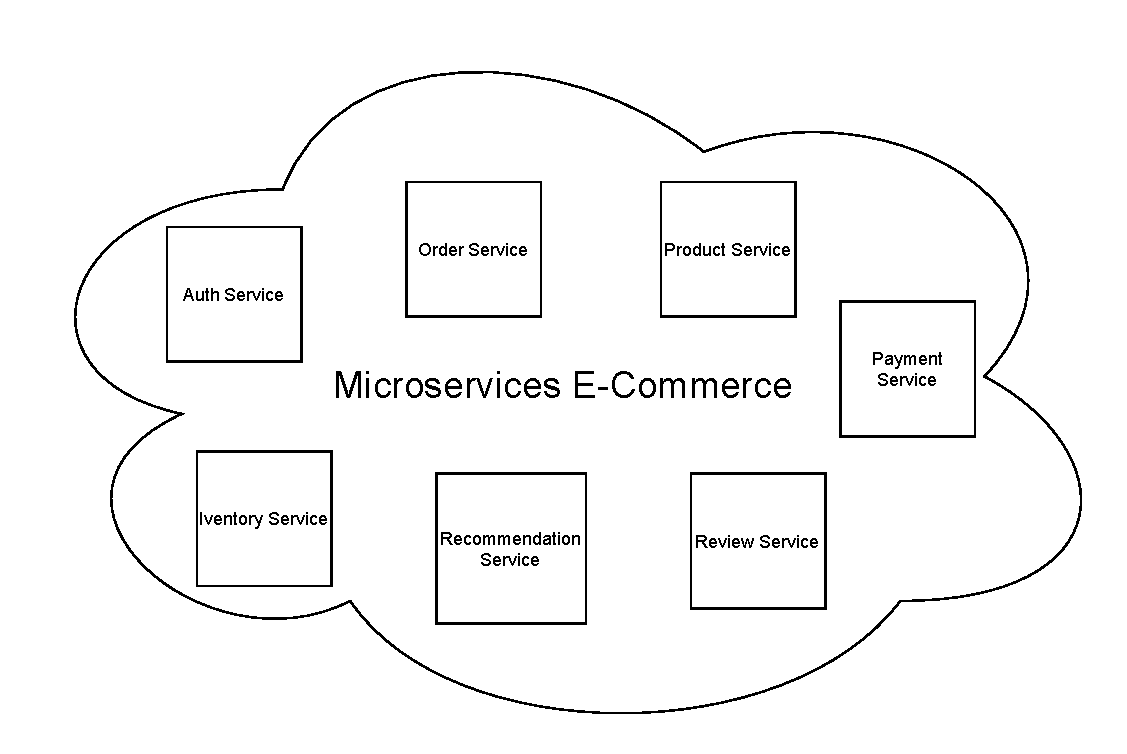
\includegraphics[width=\textwidth]{../images/Chapter-14-Studi-Kasus}
	\caption{Studi Kasus \textit{E-Commerce Microservice}.}
	\label{fig:client-server-schema}
\end{figure}
\\Fitur utama DevOps:
	\\\textit{CI/CD Pipeline} digunakan untuk melakukan \textit{compile code}, \textit{unit testing}, \textit{integration testing}, \textit{packaging}, \textit{deployment} dan \textit{monitoring}.
	Setiap kali developer melakukan \textit{push} pada \textit{repository} git, \textit{CI/CD Pipeline} otomatis melakukan \textit{compile code}, menjalankan \textit{unit tests},
	\textit{deploy} perubahan pada \textit{staging environment} untuk \textit{integration testing}. Jika \textit{integration test} dilewati, maka akan di \textit{deploy} di \textit{production environment}.
	\\Menggunakan DevOps dapat membuat developer fokus pada fitur aplikasi yang ingin dibangun sehingga tidak terlalu lama memikirkan setup infrastruktur untuk \textit{testing} dan lainnya.
\section{Code}
Code dapat dilihat di link berikut\\
\url{https://github.com/alfa-yohannis/software-architecture/tree/main/code/chapter14}

\section{Video Tutorial}
Video penjelasan mengenai proses Heroku:\\
\url{https://youtu.be/My2MOkgRPwo}